%
% Apunte de Sistemas Operativos
% Copyright (C) 2014 Esteban De La Fuente Rubio (esteban[at]delaf.cl)
%
% Permission is granted to copy, distribute and/or modify this document
% under the terms of the GNU Free Documentation License, Version 1.3
% or any later version published by the Free Software Foundation;
% with no Invariant Sections, no Front-Cover Texts, and no Back-Cover Texts.
% A copy of the license is included in the section entitled "GNU
% Free Documentation License".
%
% Link: http://www.gnu.org/copyleft/fdl.html
%

% PROTECCIÓN Y SEGURIDAD
\chapter{Protección y seguridad}
\label{proteccion}
Controlar el acceso a los recursos es una de las tareas más importantes del
sistema operativo, sin embargo no solo debe asegurar que estos accesos sean
sincronizados y sin problemas de concurrencia (como ya se discutió
anteriormente), sino que también debe asegurar que solo accedan a los recursos
quienes estén autorizados a hacerlo.

En un modelo de protección el computador simplemente es un conjunto de objetos,
ya sean estos físicos (hardware) o lógicos (software o datos). Donde cada objeto
puede ser identificado por un nombre único y tendrá asociado un conjunto
definido de operaciones.

Entonces, el problema de la protección consiste en asegurar que cada objeto sea
accedido correctamente, mediante las operaciones definidas, y solo por aquellos
procesos que tienen permitido hacerlo.

En este capítulo se hablará de conceptos de protección genéricos, los cuales
pueden aplicarse a un sistema operativo o bien a cualquier otro tipo de sistema,
ya sea o no computacional.

\section{Principios de protección}
En protección se considera generalmente el \textbf{principio del menor
privilegio}, esto implica que un programa, usuario o sistema en general deberá
tener los privilegios mínimos para poder realizar las tareas que deba hacer.

Supongamos una secretaria en un banco, sería un error dar a ella acceso a la
bóveda si de lo único que se tiene que encargar es atender las consultas de los
clientes. Para realizar su tarea, ``atender clientes'', la secretaria solo
necesita acceso a una determinada área del banco, no a todo este.

Esto tiene mucha relación con la idea de \textbf{denegar todo y permitir
algunos}, donde se evita que el usuario pueda hacer cualquier cosa en el sistema
y solo se le conceden accesos específicos según lo que debe realizar.

Este tipo de política limita el daño si la ejecución del proceso tiene algún
error, ya que de haberlo a lo más podrá afectar a aquellos objetos con los que
tenía permitido interactuar.

La forma de utilizar esta política es concediendo los privilegios de forma
\textbf{estática}, o sea el proceso durante toda su ejecución tendrá los mismos
privilegios. O bien de forma \textbf{dinámica} donde el proceso podrá cambiar
sus privilegios según vaya requiriendo, este concepto es conocido como
\textbf{escalada de privilegios}.

Se deberá determinar a que nivel de detalle se manejarán los privilegios, un
nivel más tosco implicará un manejo más simple, sin embargo se deberá realizar a
grandes rasgos o abarcando muchas operaciones u objetos. Un manejo más fino será
más complejo de administrar, pero permitirá definir con precisión los
privilegios para los procesos.

\section{Dominios}
Un dominio definirá un conjunto de derechos de acceso que el proceso (o usuario)
tienen sobre determinados objetos, especificando para cada uno de estos objetos
las posibles operaciones que el proceso puede realizar sobre el mismo.

En la figura \ref{fig:proteccion_dominios} se puede observar un ejemplo con tres
dominios, cada uno con un conjunto de derechos de acceso y las operaciones que
pueden realizar sobre cada uno de los objetos. Notar que los dominios $D_2$ y
$D_3$ comparten una misma operación sobre un objeto.

\begin{figure}[htbp]
\centering
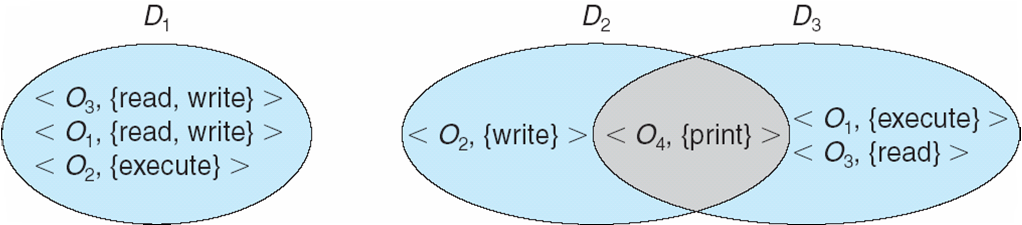
\includegraphics[scale=0.6]{img/C09_proteccion/dominios.png}
\caption{Ejemplo de dominios y sus conjuntos de derechos de acceso}
\label{fig:proteccion_dominios}
\end{figure}

\subsection{Dominios en sistemas \textit{like Unix}}
En sistemas operativos \textit{like Unix}, los dominios están definidos por el
identificador del usuario (UID) y el o los grupos a los que pertenece el usuario
(GID).

El cambio de dominio, específicamente el cambio de dominio definido por el UID,
puede ser realizado de diferentes maneras:
\begin{enumerate}[i.]

\item \textbf{Vía sistema de archivos}: cada archivo tiene asociado un bit
(\textit{setuid bit}) que permite indicar que cuando el archivo sea ejecutado se
realice con el dominio del dueño del archivo y no con el dominio de quien
ejecuta el archivo.

\item \textbf{Vía contraseñas}: comando \texttt{su} que permite cambiar a otro
dominio de usuario.

\item \textbf{Vía comandos}: comando \texttt{sudo} que ejecuta un comando
específico utilizando otro domino. Generalmente el otro dominio es el del
usuario con UID 0 (root), pero no necesariamente tiene que ser ese dominio.

\end{enumerate}

\section{Matriz de acceso}
Las políticas de protección se pueden ver como una matriz (tabla) donde las
filas representan los dominios, las columnas representan los objetos y cada
$casilla_{ij}$ de la tabla corresponde a las operaciones que un proceso
ejecutándose en el dominio $i$ puede realizar sobre el objeto $j$.

En la figura \ref{fig:matriz_acceso} se puede observar un ejemplo de una matriz
de acceso donde, por ejemplo, el dominio $D_3$ puede leer el fichero $F_2$ pero
no el $F_1$. De la misma forma el único que puede imprimir es el dominio $D_2$.

\begin{figure}[htbp]
\centering
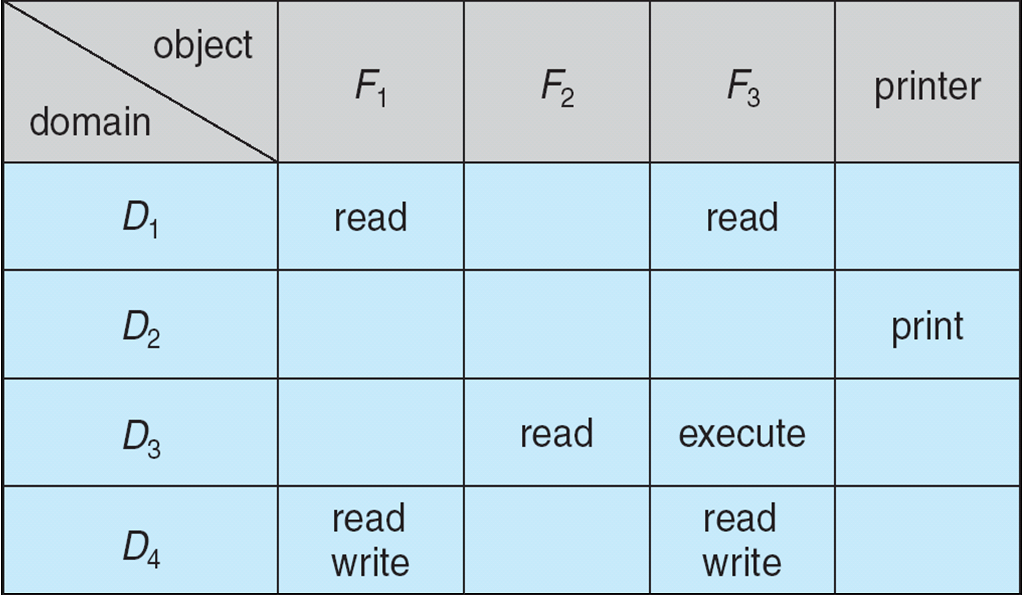
\includegraphics[scale=0.5]{img/C09_proteccion/matriz_acceso.png}
\caption{Ejemplo de matriz de acceso}
\label{fig:matriz_acceso}
\end{figure}

En general la forma de revisar la matriz de acceso es: si un proceso del dominio
$D_i$ trata de hacer una operación $X$ en el objeto $O_j$, entonces la operación
$X$ debe estar en la $casilla_{ij}$ en la matriz de acceso.

Se deben definir operaciones para agregar o quitar derechos de uso, algunas son:
\begin{itemize}
\item Definir propietario de $Objeto_j$.
\item Copiar operación desde $Objeto_j$ a $Objeto_k$.
\item Control: $Dominio_i$ puede modificar los accesos de $Dominio_h$.
\item Transferencia: del dominio $Dominio_i$ al $Dominio_h$.
\end{itemize}

Para definir las operaciones sobre dominios es necesario que el dominio sea
tratado como un objeto más dentro de la matriz de acceso, de esta forma se
tendrá algo similar al ejemplo de la figura \ref{fig:matriz_acceso_dominios}.

\begin{figure}[htbp]
\centering
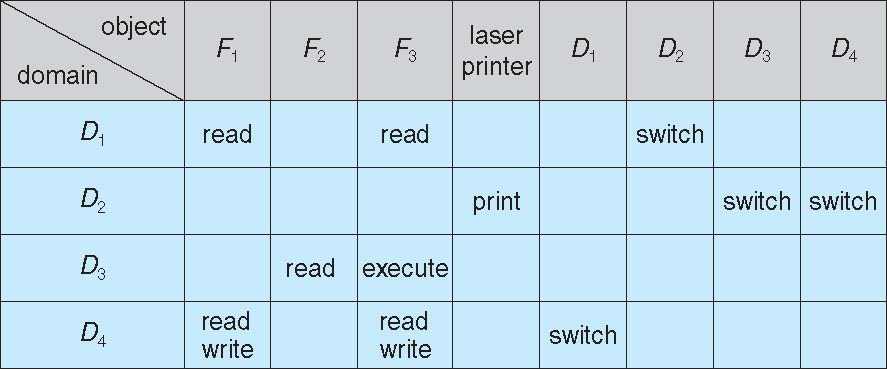
\includegraphics[scale=1.2]{img/C09_proteccion/matriz_acceso_dominios.jpg}
\caption{Ejemplo de matriz de acceso usando dominios como objetos}
\label{fig:matriz_acceso_dominios}
\end{figure}

Finalmente es importante mencionar que la matriz de acceso separa políticas de
mecanismos, teniendo que:
\begin{itemize}
\item Mecanismos:
\begin{itemize}
	\item Sistema operativo provee de matriz de acceso más reglas.
	\item Asegura que la matriz sea solo manipulada por agentes autorizados.
	\item Reglas de la matriz aplicadas estrictamente.
\end{itemize}
\item Políticas:
\begin{itemize}
	\item Usuario indica las políticas.
	\item Se define \textbf{¿quién puede acceder?} a que objeto y
	\textbf{¿en qué	modo?}.
\end{itemize}
\end{itemize}

\section{Ejercicios y preguntas}
\begin{enumerate}
\item Explique el principio del menor privilegio.
\item ¿Por qué es recomendable denegar todo y solo asignar los permisos
específicos que son requeridos?
\item Explique los métodos de asignación de privilegios estáticos y dinámicos.
\item ¿En qué consisten los dominios?.
\item ¿Qué son los derechos de acceso?.
\item ¿Cuáles son las tres vías para hacer un cambio de dominio en Unix?.
\item ¿Qué es la matriz de acceso?.
\item ¿Qué representan las filas y columnas en la matriz de acceso?.
\item ¿Por qué se podría querer tratar a los dominios como objetos en la matriz
de acceso?.
\end{enumerate}

\section{Referencias}
\begin{itemize}
\item Sistemas Operativos, Quinta Edición, Abraham Silberschatz y Peter Baer
Galvin, Capítulo 19 y 20.
\item Sistemas Operativos, Segunda Edición, William Stallings, Capítulo 14.
\end{itemize}
